\documentclass[class=article,border=5pt,tikz]{standalone}

\begin{document}
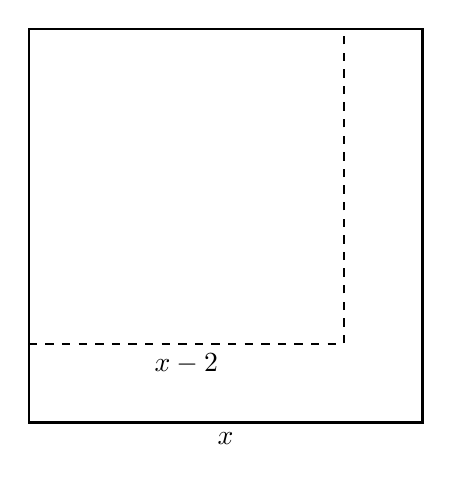
\begin{tikzpicture}[thick,x=1cm,y=1cm]
\coordinate (A) at (0,0);
\coordinate (B) at (5,0);
\coordinate (C) at (5,5);
\coordinate (D) at (0,5);
\coordinate (E) at (0,1);
\coordinate (F) at (4,1);
\coordinate (G) at (4,5);
\draw (A) -- (B) -- (C) -- (D) -- cycle;
\draw [dashed] (E) -- (F) -- (G);
\path (A) -- (B) node[midway, below] {$x$};
\path (E) -- (F) node[midway, below] {$x-2$};
\end{tikzpicture}
\end{document}

